\section{Натуральный триэдр. Проекции ускорения точки на оси натурального
триэдра}

\subsection{Натуральный триэдр траектории}

\begin{figure}[H]
  \centering
  \resizebox{\linewidth}{!}{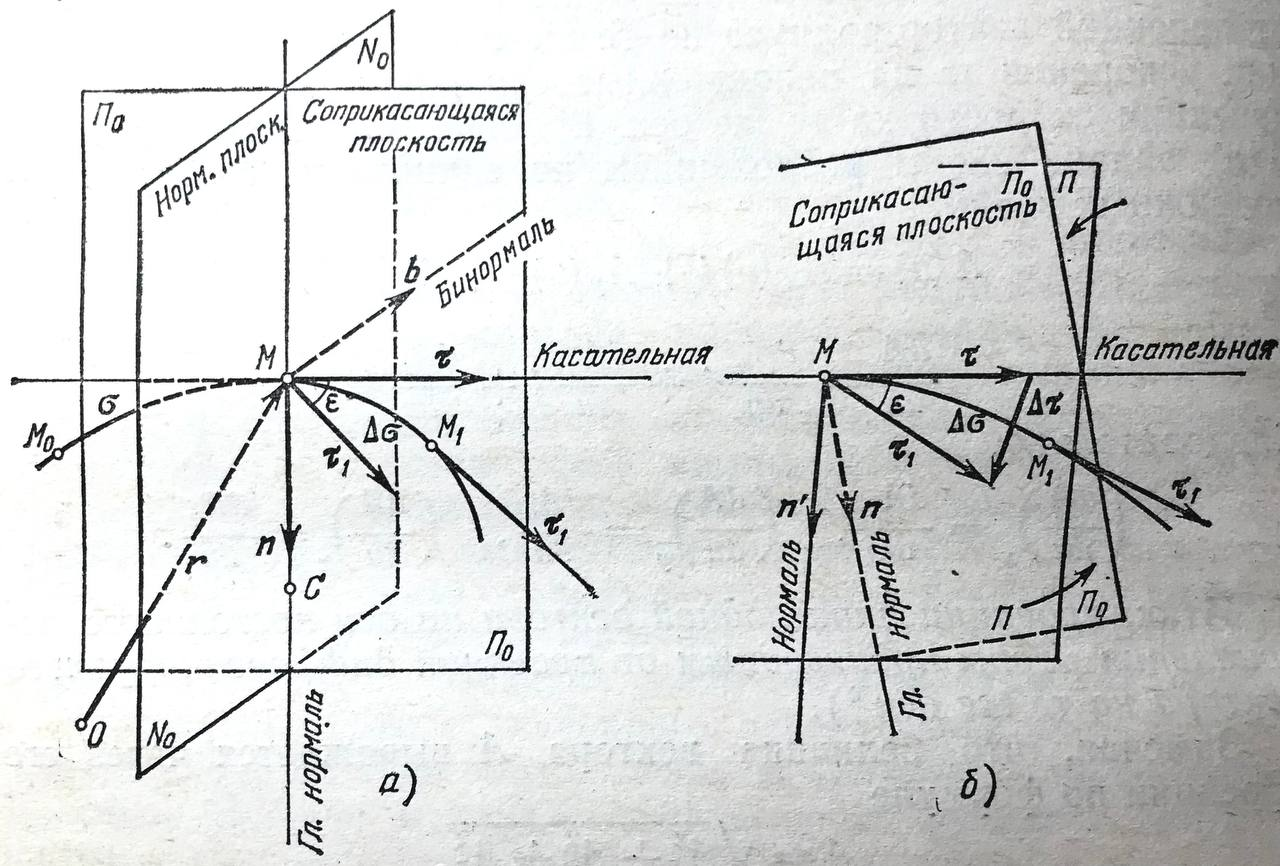
\includegraphics{src/mechanics/pictures/7_1.jpg}}

  \caption{}
  \label{fig:natural_trihedron}
\end{figure}

Рассмотрим некоторую кривую, не лежащую в одной плоскости (кривую двоякой
кривизны). Установим на этой кривой начало $M_0$ и положительное направление
отсчёта дуг $\sigma$. Возьмём какую-нибудь текущую точку $M$, положение
которой определим либо дугой $\sigma$, либо вектор-радиусом $\xvec{r}$
относительно некоторой неподвижной точки $O$. Через точку $M$ проведём
касательную к кривой; направление касательной в сторону возрастающих значений
$\sigma$ зададим единичным вектором касательной $\xvec{\tau}$.

Возьмём на кривой весьма близкую к $M$ точку $M_1$; пусть положение её
определяется значением дуги $\sigma + \Delta \sigma$, причём
$\Delta \sigma > 0$, то есть $M_1$ лежит за $M$ в сторону положительного
отсчёта дуги. Единичный вектор касательной в точке $M_1$ обозначим через
$\xvec{\tau}_1$. Проведём через $\xvec{\tau}$ плоскость $\Pi$, параллельную
$\xvec{\tau}_1$; чтобы построить её, достаточно перенести $\xvec{\tau}_1$ в
точку $M$; два вектора $\xvec{\tau}$ и $\xvec{\tau}_1$, имеющие начало в точке
$M$, определяют положение $\Pi$. При изменении положения $M_1$ плоскость $\Pi$
также изменяет своё положение, вращаясь вокруг $\xvec{\tau}$; если будем
приближать $M_1$ к $M$, уменьшая $\Delta \sigma$ до нуля, то эта плоскость
будет приближаться к некоторому предельному положению $\Pi_0$, называемому
\textit{соприкасающейся плоскостью}.

В точке $M$ проведём плоскость $N_0$, перпендикулярную к касательной. Эта
плоскость называется \textit{нормальной плоскостью} кривой. Любая прямая,
проведённая в этой плоскости через точку $M$, будет перпендикулярна к
$\xvec{\tau}$, то есть будет \textit{нормальна} кривой; линия пересечения
нормальной и соприкасающейся плоскостей определяет \textit{главную нормаль}
кривой. Иными словами, главной нормалью называется нормаль, лежащая в
соприкасающейся плоскости. Нормаль, перпендикулярная к главной нормали,
называется \textit{бинормалью} кривой.

\begin{definition}
  Совокупность трёх взаимно перпендикулярных осей:
  \begin{enumerate}
    \item касательной, направленной в сторону возрастания дуги,
    \item главной нормали, направленной в сторону вогнутости кривой, и
    \item бинормали, направленной по отношению к касательной и главной нормали
      так же, как ось $Oz$ расположена по отношению к осям $Ox$ и $Oy$,
  \end{enumerate}
  образует так называемый \textit{натуральный триэдр}
  (естественный трёхгранник) кривой. Единичные векторы этих осей обозначим
  соответственно через $\xvec{\tau}, \xvec{n}$ и $\xvec{b}$.
\end{definition}

Найдём выражения этих трёх единичных векторов натурального триэдра через
вектор-радиус точки на кривой, заданный как вектор-функция дуги:
\begin{equation}
  \xvec{r} = \xvec{r}(\sigma).
\end{equation}

Найдём прежде всего $\xvec{\tau}$. По определению векторной производной вектор
${\displaystyle \diff{\xvec{r}}{\sigma}}$ направлен по касательной к годографу
вектора $\xvec{r}$ в сторону возрастающих $\sigma$. С другой стороны, численная
величина производной равна
\begin{equation*}
  \abs{\diff{\xvec{r}}{\sigma}} = \frac{\abs{\dd{\xvec{r}}}}{\dd{\sigma}} = 1.
\end{equation*}
Таким образом, векторная производная представляет собой искомый единичный
вектор касательной:
\begin{equation}
  \xvec{\tau} = \diff{\xvec{r}}{\sigma}.
\end{equation}

Для определения единичного вектора главной нормали $\xvec{n}$ обратимся к
рисунку. Рассмотрим равнобедренный треугольник, образованный векторами
$\xvec{\tau}$ и $\xvec{\tau}_1$ в плоскости $\Pi$. Если точка $M_1$ взята на
весьма малом расстоянии $\Delta \sigma$ от точки $M$, то угол $\varepsilon$
между касательными $\xvec{\tau}$ и $\xvec{\tau}_1$ в смежных точках кривой ---
его называют \textit{углом смежности} --- будет также мал и вектор
$\Delta \xvec{r}$ с тем меньшей ошибкой, чем меньше $\Delta \sigma$, можно
считать перпендикулярным к $\xvec{\tau}$ и, следовательно, параллельным вектору
нормали $\xvec{n}'$, лежащему с $\Delta \xvec{\tau}$ в одной и той же плоскости
$\Pi$. По величине $\abs{\Delta \xvec{\tau}}$, как основание равнобедренного
треугольника с малым углом $\varepsilon$ при вершине и боковыми сторонами,
равными единице, будет равен
\begin{equation*}
  \abs{\Delta \xvec{\tau}} = 2 \abs{\xvec{\tau}} \sin \frac{\varepsilon}{2}
    \approx 2 \cdot 1 \cdot \frac{\varepsilon}{2} = \varepsilon.
\end{equation*}
Отсюда найдём (с точностью до малых высших порядков)
\begin{equation*}
  \Delta \xvec{\tau} = \varepsilon \xvec{n}',
\end{equation*}
или
\begin{equation*}
  \xvec{n}' = \frac{1}{\varepsilon} \Delta \xvec{\tau} =
    \frac{\Delta \xvec{\tau}}{\Delta \sigma} \cdot
    \frac{\Delta \sigma}{\varepsilon}.
\end{equation*}
Будем приближать $\Delta \sigma$ к нулю, тогда точка $M_1$ будет стремиться к
$M$, плоскость $\Pi$ --- к соприкасающейся плоскости $\Pi_0$, единичный вектор
нормали $\xvec{n}'$ --- к искомому единичному вектору $\xvec{n}$, и мы будем
иметь
\begin{equation*}
  \xvec{n} = \lim_{\Delta \sigma \to 0} \frac{\Delta \xvec{\tau}}{\Delta \sigma}
    \cdot \lim_{\Delta \sigma \to 0} \frac{\Delta \sigma}{\varepsilon}.
\end{equation*}

Первый предел равен векторной производной
\begin{equation*}
  \diff{\xvec{\tau}}{\sigma} = \diff{}{\sigma} \paren{\diff{\xvec{r}}{\sigma}} =
    \diff[2]{\xvec{r}}{\sigma};
\end{equation*}
что же касается второго предела, то заметим, что отношение
$\dfrac{\varepsilon}{\Delta \sigma}$, определяющее среднюю скорость поворота
касательной к кривой при переходе от данной точки к смежной, характеризует
\textit{среднюю кривизну} кривой на участке $(\sigma, \sigma + \Delta \sigma)$,
а величина
\begin{equation}
  \lim_{\Delta \sigma \to 0} \frac{\varepsilon}{\Delta \sigma} = K
\end{equation}
определяет \textit{кривизну} кривой в данной точке.

Таким образом, имеем следующее выражение единичного вектора \textit{главной
нормали}:
\begin{equation}
  \label{eq:main_norm}
  \xvec{n} = \frac{1}{K} \diff{\xvec{\tau}}{\sigma} = \frac{1}{K}
    \diff[2]{\xvec{r}}{\sigma}.
\end{equation}
Величину $1/K = \rho$, имеющую размерность длины, называют \textit{радиусом
кривизны} кривой в данной точке.

В случае произвольной кривой через данную её точку и две смежные с нею точки
можно провести круг, который при стремлении смежных точек к данной
рассматриваемой будет стремиться к некоторому предельному кругу, называемому 
\textit{соприкасающимся кругом} или \textit{кругом кривизны}. Радиус этого круга
будет радиусом кривизны кривой, центр круга $C$ --- \textit{центром кривизны}
кривой. Очевидно, круг кривизны лежит в соприкасающейся плоскости, центр
кривизны $C$ --- на главной нормали со стороны вогнутости кривой.

Введя радиус кривизны $\rho$, получим
\begin{equation}
  \xvec{n} = \rho \diff{\xvec{\tau}}{\sigma} = \rho \diff[2]{\xvec{r}}{\sigma}.
\end{equation}

Теперь уже не составляет труда найти и единичный вектор бинормали. Из условия
выбора положительного направления на бинормали следует:
\begin{equation}
  \xvec{b} = \crossprod{\xvec{\tau}}{\xvec{n}} = \frac{1}{K}
  \paren{\crossprod{\diff{\xvec{r}}{\sigma}}{\diff[2]{\xvec{r}}{\sigma}}} = \rho
  \paren{\crossprod{\diff{\xvec{r}}{\sigma}}{\diff[2]{\xvec{r}}{\sigma}}}.
\end{equation}

\subsection{Разложение ускорения по осям натурального триэдра траектории}

Обозначим через $v_\tau$ проекцию вектора скорости на направление касательной
к траектории. Очевидно, что $v_\tau$ по абсолютной величине равно численной
величине скорости $v$; что же касается знака $v_\tau$, то $v_\tau$ положительно,
если направление движения в данный момент совпадает с направлением
положительного отсчёта дуг $\sigma$ по траектории, и отрицательно в
противоположном случае. Будем иметь
\begin{equation}
  \label{eq:vel_natural}
  \xvec{v} = v_\tau \xvec{\tau}.
\end{equation}

Если $s$ --- пройденный путь, то $\dd{\sigma} = \dd{s}$, когда
$\dd{\sigma} > 0$, и $\dd{\sigma} = -\dd{s}$, если $\dd{\sigma} <0$, поэтому
\begin{equation}
  \label{eq:v_tau}
  v_\tau = \dt[\sigma] = \pm \dt[s] = \pm v.
\end{equation}

Вектор ускорения есть производная по времени от вектора скорости, поэтому
\begin{equation}
  \label{eq:acc_natural_temp}
  \xvec{w} = \dt[\xvec{v}] = \dt (v_\tau \xvec{\tau}) = \dt[v_\tau] \xvec{\tau} +
    v_\tau \dt[\xvec{\tau}].
\end{equation}

Далее, имеем
\begin{equation*}
  \dt[\xvec{\tau}] = \diff{\xvec{\tau}}{\sigma} \dt[\sigma];
\end{equation*}
согласно формулам \ref{eq:main_norm} и \ref{eq:v_tau} найдём
\begin{equation*}
  \dt[\xvec{\tau}] = \frac{1}{\rho} \xvec{n} v_\tau.
\end{equation*}

Подставив полученное выражение в равенство \ref{eq:acc_natural_temp}, будем
иметь
\begin{equation}
  \label{eq:acc_natural}
  \xvec{w} = \xvec{\tau} \dt[v_\tau] + \xvec{n} \frac{v^2}{\rho},
\end{equation}
где $v_\tau^2$ заменено на равное ему $v^2$.

Равенство \ref{eq:acc_natural} представляет собой \textit{разложение вектора
ускорения по осям натурального триэдра}.

Обозначим коэффициенты при единичных векторах $\xvec{\tau},~\xvec{n}$ и $\xvec{b}$
в разложении \ref{eq:acc_natural}, то есть проекции ускорения на оси
натурального триэдра, соответственно через $w_\tau,~w_n$ и $w_b$; тогда будем
иметь
\begin{equation}
  \label{eq:acc_natural_general}
  \xvec{w} = w_\tau \xvec{\tau} + w_n \xvec{n} + w_b \xvec{b},
\end{equation}
причём из \autoref{eq:acc_natural} следует, что
\begin{equation*}
  w_\tau = \dt[v_\tau] = \ddt[\sigma], \quad w_n = \frac{v^2}{\rho},
    \quad w_b = 0.
\end{equation*}

Последнее равенство говорит о том, что вектор ускорения перпендикулярен к
бинормали, то есть \textit{ускорение лежит в соприкасающейся плоскости}.

Первое слагаемое в разложении \ref{eq:acc_natural_general}, $w_\tau \xvec{\tau}$,
даёт \textit{касательную} (тангенциальную) составляющую ускорения, второе, $w_n
\xvec{n}$, --- \textit{нормальную} составляющую ускорения. Иногда для краткости
их называют просто касательным и нормальным ускорениями.

Нормальное ускорение всегда совпадает по направлению с главной нормалью, так как
$w_n = \dfrac{v^2}{\rho}$ --- существенно положительная величина. Вспоминая
ранее сказанное о направлении $\xvec{n}$, видим, что \textit{нормальное ускорение
направлено к центру кривизны траектории} (нормальное ускорение иногда ещё
называют поэтому \textit{центростремительным}), то есть по главной нормали к
траектории в сторону её вогнутости. Отсюда вытекает свойство ускорения:
\textit{вектор ускорения направлен в сторону вогнутости траектории}.

Итак, \textit{вектор ускорения в криволинейном движении может быть представлен
как геометрическая сумма двух ускорений: касательного и нормального}.

Величина ускорения может быть представлена так:
% TODO: dv/dt или dv_\tau/dt?
\begin{equation}
  w = \sqrt{w_\tau^2 + w_n^2} =
    \sqrt{\paren{\dt[v]}^2 + \frac{v^4}{\rho^2}},
\end{equation}
а направление задано косинусами углов, составляемых им с касательной и главной
нормалью к траектории:
\begin{equation}
  \cos(\widehat{\xvec{w}, \xvec{\tau}}) = \frac{w_\tau}{w}, \quad
  \cos(\widehat{\xvec{w}, \xvec{n}}) = \frac{w_n}{w}.
\end{equation}

\subsection{Список литературы}
\begin{enumerate}
  \item \cite{lourie}
\end{enumerate}

